\documentclass[11pt]{article}
\usepackage{icmlko}
\begin{document}

\title{안은 정보를 주고 밖은 눈금을 준다 --- 한 도메인 안에서 갈라 확인했다}
\author{월드모델 실험실}
\date{노트 391 · 2026년 8월 1일}
\maketitle

\begin{abstract}
노트 390이 점 셋으로 대응을 하나 봤다 --- \emph{새 학습 행 중 기존 범위
밖 비율}과 \emph{위약이 남기는 이득 비율}이 거의 같다(10/$-8$ · 16/7.5 ·
100/91). 그리고 ``16\%와 100\% 사이가 비어 있으니 그 사례가 나와야 진짜인지
안다''고 적었다.

\textbf{가운데 점을 모으려다 실패했다.} 만화에서 학습 바닥(5,306)을 걸치는
구간을 받으려 했는데, AniList 에서 받을 수 있는 새 행이 전부 그 아래였다
(2,390\,--\,5,308, 밖 100\%). 우리 만화 학습이 이미 목록 꼭대기라 걸칠 데가
없다.

\textbf{그래서 점을 모으는 대신 기제를 갈랐다.} 노트 381이 펀딩에 더한
2,038행을 \emph{기존 범위 안}(1,712행 · 84\%)과 \emph{밖}(326행 · 16\%)으로
나눠, 각각 따로 넣고 각각 위약을 붙였다. 사전 등록: \emph{안 쪽은 위약이
이득을 지우고 밖 쪽은 못 지운다.}

\begin{center}
\begin{tabular}{lrrrr}
\hline
 & 실제 & 부호 & 위약 & 잔량 \\
\hline
안 (84\% · 1,712행) & $+0.1582$ & 12/12 & $\mathbf{-0.0371}$ & $\mathbf{-23\%}$ \\
밖 (16\% · \,\,\,326행) & $+0.1091$ & 12/12 & $\mathbf{+0.1138}$ & $\mathbf{104\%}$ \\
\hline
\end{tabular}
\end{center}

\textbf{사전 등록대로다.} 같은 도메인 · 같은 유보 · 같은 축에서 새 행을
어느 쪽에서 골랐느냐만 바꿨는데 위약의 운명이 정반대다. \textbf{안의 새 행은
정보를 주고, 밖의 새 행은 눈금을 준다.}

그리고 이것이 노트 381을 가른다: 판 $+0.0348$ 중 안이 $+0.0243$ · 밖이
$+0.0161$ 이다 --- \textbf{그 이득의 46\%는 정보가 아니라 눈금이었다.}

\textbf{그래도 밖 326행을 안 뺀다.} 조항 ⑤는 \emph{이득을 주장하는 것}을
막는 규칙이지 \emph{자료를 고르는} 규칙이 아니다. 밖의 326행은 노트 379가
고친 대표성의 일부라, 빼면 학습이 다시 위로 쏠린다. \textbf{조항 ⑤를 자료
결정에 적용하면 편향을 되돌리라는 말이 된다.}
\end{abstract}

\section{가운데 점은 못 모았다}

노트 390의 대응을 시험하려면 밖 비율이 30\,--\,70\%인 사례가 필요하다.
만화 학습 라벨 최소가 5,306 이므로 그 위아래를 걸치는 구간
(popularity 2,000\,--\,20,000)을 받으면 될 것 같았다.

받아 보니 새 행 3,045편이 popularity 2,390\,--\,5,308 로 \textbf{전부 학습
최소 아래}다. 이유는 단순하다 --- 우리 만화 표본이 이미 목록 상위 3,000이라
5,306 위에 남은 것이 거의 없다. \textbf{걸칠 데가 없으니 걸치는 표본도
없다.} 다른 도메인에서 30\,--\,70\% 사례를 찾는 것은 남겨 둔다.

\begin{figure}[t]
\centering
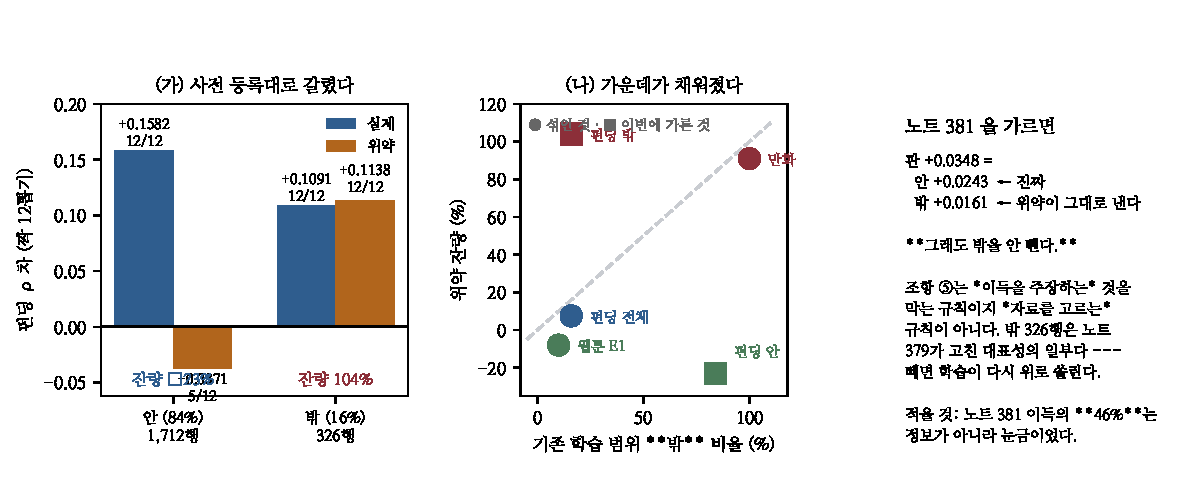
\includegraphics[width=\linewidth]{figs/fig391.pdf}
\caption{\textbf{(가)} 펀딩의 더한 행을 안/밖으로 갈라 각각 위약을 붙였다.
안은 위약이 이득을 지우고(잔량 $-23$\%) 밖은 그대로 낸다(104\%).
\textbf{(나)} 노트 390의 점 셋(원)에 이번에 가른 둘(네모)이 붙었다.
\textbf{(다)} 노트 381의 이득 분해.}
\label{fig:main}
\end{figure}

\section{점 대신 기제를 갈랐다}

노트 390의 대응은 도메인 사이 비교라 다른 것이 스무 가지 같이 움직인다.
\textbf{한 도메인 안에서 가르면 그것들이 상수가 된다.}

펀딩에서 노트 381이 더한 2,038행을 기존 학습 라벨 범위
($10^{0.954}{=}9$ \,--\, $10^{4.004}{=}10{,}090$ 후원자)로 갈랐다 ---
안 1,712행 · 밖 326행. 팔 다섯을 만들었다: 아무것도 안 넣은 A, 안만 넣은 B와
그 위약 C, 밖만 넣은 D와 그 위약 E. 유보 529행은 다섯이 전부 같다.

\begin{center}
\begin{tabular}{lrrrr}
\hline
A 대비 & 판 차 & 부호 & 펀딩 차 & 부호 \\
\hline
B 안 (84\%) & $+0.0243$ & 12/12 & $+0.1582$ & 12/12 \\
C 안 위약 & $-0.0056$ & 5/12 & $-0.0371$ & 5/12 \\
D 밖 (16\%) & $+0.0161$ & 12/12 & $+0.1091$ & 12/12 \\
E 밖 위약 & $+0.0165$ & 12/12 & $+0.1138$ & 12/12 \\
\hline
\end{tabular}
\end{center}

\textbf{D와 E가 넷째 자리까지 같다.} 밖의 326행은 어느 행에 어느 라벨이
붙었는지가 아무 값이 없다 --- 그 구간이 존재한다는 사실만 전달한다. 반대로
C는 A보다 \emph{아래}로 간다: 안의 1,712행에서 라벨을 섞으면 이득이
사라지는 정도가 아니라 잡음을 더한다.

\textbf{기제가 확인됐다:} 기존 범위 안의 새 행은 \emph{그 구간을 촘촘히}
해서 어느 축이 어느 라벨과 가는지를 더 정확히 알려 준다(섞으면 없어진다).
밖의 새 행은 \emph{그 구간이 있다}를 알려 주고 그것은 라벨 배치와 무관하다
(섞어도 남는다).

\section{그래서 노트 381을 어떻게 읽나}

\begin{center}
판 $+0.0348$ \; = \; 안 $+0.0243$ (정보) \; $+$ \; 밖 $+0.0161$ (눈금)
\end{center}

\textbf{노트 381이 보고한 이득의 46\%가 정보가 아니었다.} 노트 390이 전체
위약으로 ``잔량 7.5\%''를 얻은 것은 안의 음수 잔량($-23$\%)과 밖의 양수
잔량(104\%)이 상쇄된 값이었다 --- \textbf{섞어서 재면 상쇄돼 보인다.}
조항 ⑤를 돌릴 때 안/밖을 갈라 보는 것이 낫다.

\textbf{그런데 밖 326행을 빼지는 않는다.} 이유가 셋이다.

\textbf{첫째, 조항 ⑤의 관할이 다르다.} 그 조항은 ``이 변경이 판을
올렸다''는 \emph{주장}을 검증한다. 밖의 326행이 판을 올린 것은 사실이고
(D $+0.0161$ · 12/12) 다만 그 이유가 정보가 아닐 뿐이다. 자료를 넣을지는
노트 82 · 90의 분모 규칙이 정하고, 그 규칙은 재현성과 대표성을 본다.

\textbf{둘째, 빼면 편향이 돌아온다.} 밖의 326행은 후원자 1\,--\,8명짜리
프로젝트들이고, 노트 379가 밝힌 ``우리 표본은 목록 위 19\%''를 고치는
바로 그 부분이다. 빼면 학습이 다시 위로 쏠린다. \textbf{조항 ⑤를 자료
결정에 적용하면 편향을 되돌리라는 말이 된다.}

\textbf{셋째, 눈금이 틀린 것은 아니다.} 밖의 행들이 알려 주는 ``후원자
한 자리수 프로젝트가 존재한다''는 참이다. 모형이 그걸 알아서 예측 눈금이
옮겨 가는 것은 과적합이 아니라 교정이다. 위약이 같은 값을 내는 것은
\emph{그 정보가 라벨 배치에 안 실려 있다}는 뜻이지 \emph{가짜}라는 뜻이
아니다.

\textbf{조항 ⑤를 고쳐 적는다:} 학습 행을 더해 \emph{이득을 주장}할 때는
위약이 그 이득을 지워야 한다. 지우지 못하면 그 몫은 ``정보''가 아니라
``눈금''으로 기록하고, \emph{자료를 넣을지는 따로 분모 규칙으로 정한다.}

\section{남은 것}

\begin{center}
\begin{tabular}{lll}
\hline
항목 & 왜 값이 큰가 & 어떻게 \\
\hline
가운데 점 & 30\,--\,70\% 사례가 여전히 없다 & 애니가 받아지면 거기서 \\
지난 채택 안/밖 분해 & 웹툰 835도 섞여 있다 & 같은 다섯 팔 설계 \\
애니 아카이브 & 무게 606 · 덮음 22\% & 수집 중(500/3,000) \\
눈금 몫을 따로 적기 & 대장이 정보와 눈금을 안 나눈다 & 관문 스크립트에 안/밖 분해 \\
\hline
\end{tabular}
\end{center}

\end{document}
